\section{Convex Piecewise Likelihoods}
\label{sec:piecewise}

The linear algebraic solution to recover parameters presented in the
  previous section is efficient and easy to understand. 
However, it is sensitive to noise. 
In this section we propose an alternate solution; optimize the piecewise
  likelihoods.
We show that, under the conditions presented earlier\reword, the
  piecewise likelihoods are in fact strictly convex, guaranteeing that
  gradient-based optimization will converge to a global solution.

\paragraph{Motivation}

\begin{figure}
  \centering
  \label{fig:piecewise-objective}
  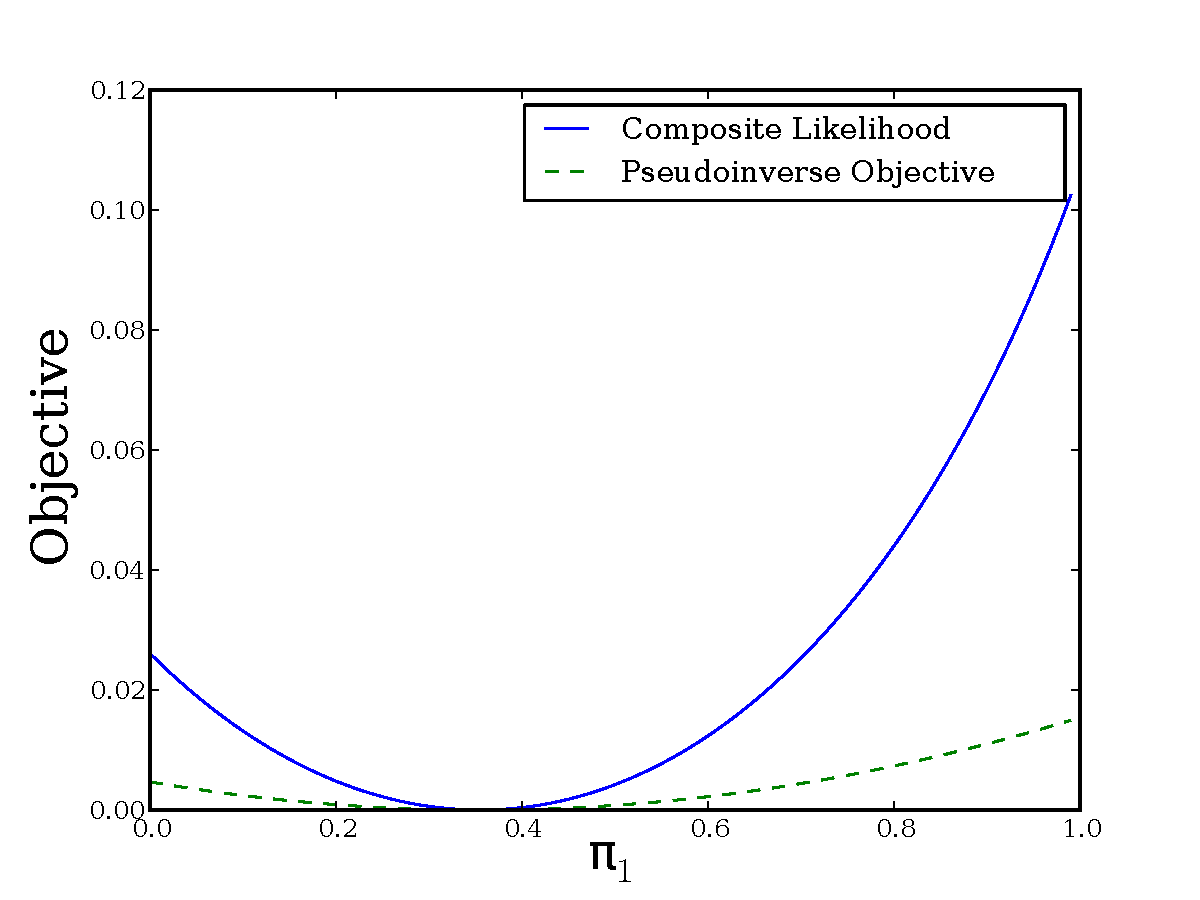
\includegraphics[width=\columnwidth]{figures/piecewise-objective.pdf}
  \caption{Comparing the piecewise objective with the moment-matching objective for just one parameter}
\end{figure}

The negative log-likelihood is more convex than the moment-reconstruction loss (\figureref{piecewise-objective})

\begin{corollary}
  The asymptotic variance of optimizing the log-likelihood, $\Sigma_p$
  is strictly less than that of the moment-matching objective
  $\Sigma_m$; $\Sigma_p \succ \Sigma_m \succ 0$.
\end{corollary}

For part two of our algorithm, we must identify the clique potentials between the
  hidden variables. 
Consider a clique $\sC = \{h_1, \cdots, h_m\}$. 
Define $\vec x_\sC = \Union_{h \in \sC} \sB(h)$ to be the collection of
  participating observed variables for this clique.
The piecewise log-likelihood of $\vec x_{\sC} =\sB(\sC)$ can then be
  written down as,
\begin{align}
  \sL_p(\vec x_\sC) 
    &= \E_{\vec x_\sC}[ \sum_{h_1, h_2, \ldots, h_m} P(h_1, h_2, \cdots, h_m) 
    \prod_{i=1}^{m} O_{h_i}(\vec x_{\sB(h_i)}) ]. \label{eqn:piecewise}
\end{align}
As we saw earlier, this objective is convex in the marginal distribution
  $P(h_1, h_2, \cdots, h_m)$, which implies that
  expectation-maximization in step 2 converges to a global optimum.
The following lemma describes conditions under which the piecewise
  likelihood objective is strongly convex, guaranteeing that the global
  optimum is unique.

  \begin{lemma} (Strict convexity of \equationref{piecewise})
  \label{lem:hessian}

  Let $\vec x_{\sC} \eqdef\{x_1, x_2, \cdots, x_L\}$. The Fisher information
  matrix $J_\sC$ for the piecewise objective in \equationref{piecewise} at the
  true parameters is 
  \begin{align}
    \grad^2 \sL_p(\vec x_\sC) 
    &= \sum_{x_1, x_2, \ldots, x_L} \tilde O_{\vec x_\sC} \tilde O_{\vec x_\sC}^T,
  \end{align}
  where $\tilde O \in \Re^{K^m \times D^L}$ is the matrix constructed as follows,
  \begin{align}
    \tilde O_{\sC, \vec x_\sC} &= O_{h_1}(\vec x_{\sB(h_1)} O_{h_2}(\vec x_{\sB(h_2)} \cdots O_{h_m}(\vec x_{\sB(h_m)}).
  \end{align}

  Consequently, the Fisher matrix is non-singular iff the span of $D^L$ vectors $\{ O_{\vec x_\sC} \}$ is rank-deficient.
  Furthermore, the smallest singular value of $J_\sC$ is bounded below
    by \todo{condition}.
\end{lemma}
\begin{proof}
  Rewrite $\sL_p$ as inner product.

  Differentiate twice.

  Observed denominators cancel at the true parameters.

  Finally, the Fisher information matrix $J_\sC$ for the piecewise
  objective in \equationref{piecewise} at the true parameters is 
  \begin{align}
    \grad^2 \sL_p(\vec x_\sC) 
    &= \sum_{x_1, x_2, \ldots, x_L} \tilde O_{\vec x_\sC} \tilde O_{\vec x_\sC}^T,
  \end{align}
  where $\tilde O \in \Re^{K^m \times D^L}$ is the matrix constructed as follows,
  \begin{align}
    \tilde O_{\sC, \vec x_\sC} &= O_{h_1}(\vec x_{\sB(h_1)} O_{h_2}(\vec x_{\sB(h_2)} \cdots O_{h_m}(\vec x_{\sB(h_m)}).
  \end{align}

  Consequently, the Fisher matrix is non-singular iff the span of $D^L$
    vectors $\{ O_{\vec x_\sC} \}$ is rank-deficient.
\end{proof}

Intuitively, the condition \todo{(C1)} says that the observations give
  us sufficient information about the latent variables to identify the
  model. 
For example, when each observed symbol corresponds to exactly one value
  of the hidden variable, i.e. $P(x \mid h )$ is binary, the above
  condition trivially holds\verify.
\todo{Is this condition the weakest possible? Can we hope to identify a model for which this is not true?}.

As a special case, suppose each hidden variable $h \in \sC$ had
  a distinct observed variable $x \in \sB(h)$. 
Then $\tilde O = O_{h_1} \otimes O_{h_2} \cdots \otimes O_{h_m}$, which
  has singular values $\sigma_1(O_{h_1}) \sigma_1(O_{h_2}) \cdots
  \sigma_1(O_{h_m}), \cdots, \sigma_k(O_{h_1}) \sigma_k(O_{h_2}) \cdots
  \sigma_k(O_{h_m})$. 
Thus, the smallest singular value is of the order $\sigma_k(O)^m$; as
  expected, the more variables in a clique, the more sensitive the
  estimation problem is to noise.
If two hidden variables $h_1, h_2$ share the same bottleneck
  variables, i.e. $\sB(h_1) = \sB(h_2)$, then we must have more
  observations in order to tease apart the effect of the two
  variables\verify\reword.


Next, we appeal to the delta method\findcite{van de vaart} to give us
  consistency and asymptotic rates on sample complexity.
\begin{corollary}(Consistency and Asymptotic Complexity)
  \label{cor:asymptotics}
  Step 2 of \algorithmref{directed} is a consistent estimator for
  the clique potential for every clique $\sC$.

  Furthermore, the asymptotic variance of $\theta_{\sC}$ is
  \todo{condition}.
\end{corollary}

Finally, coupled with \theoremref{three-view}, we can guarantee that
  \algorithmref{directed} is a consistent estimator for $\theta$ and 
  that has polynomial computational and sample complexity.
\begin{theorem}
  \algorithmref{directed} is a consistent estimator for $\theta$.
  Furthermore, it has a computational complexity of \todo{$O(?)$} and an
    asymptotic sample complexity of \todo{$O(?)$}.
\end{theorem}
\begin{proof}
  \todo{Staple together \theoremref{three-view} and \corollaryref{cor:asymptotics}}.
\end{proof}
